% !TeX spellcheck = it_IT

\section{Vulnerabilities Detection}

Dato un programma, si vuole cercare in modo proattivo se sono presenti vulnerabilità. Esistono molti metodi per cercare vulnerabilità, che possono essere più o meno automatici e possono operare in maniera statica o dinamica.
\begin{center}
	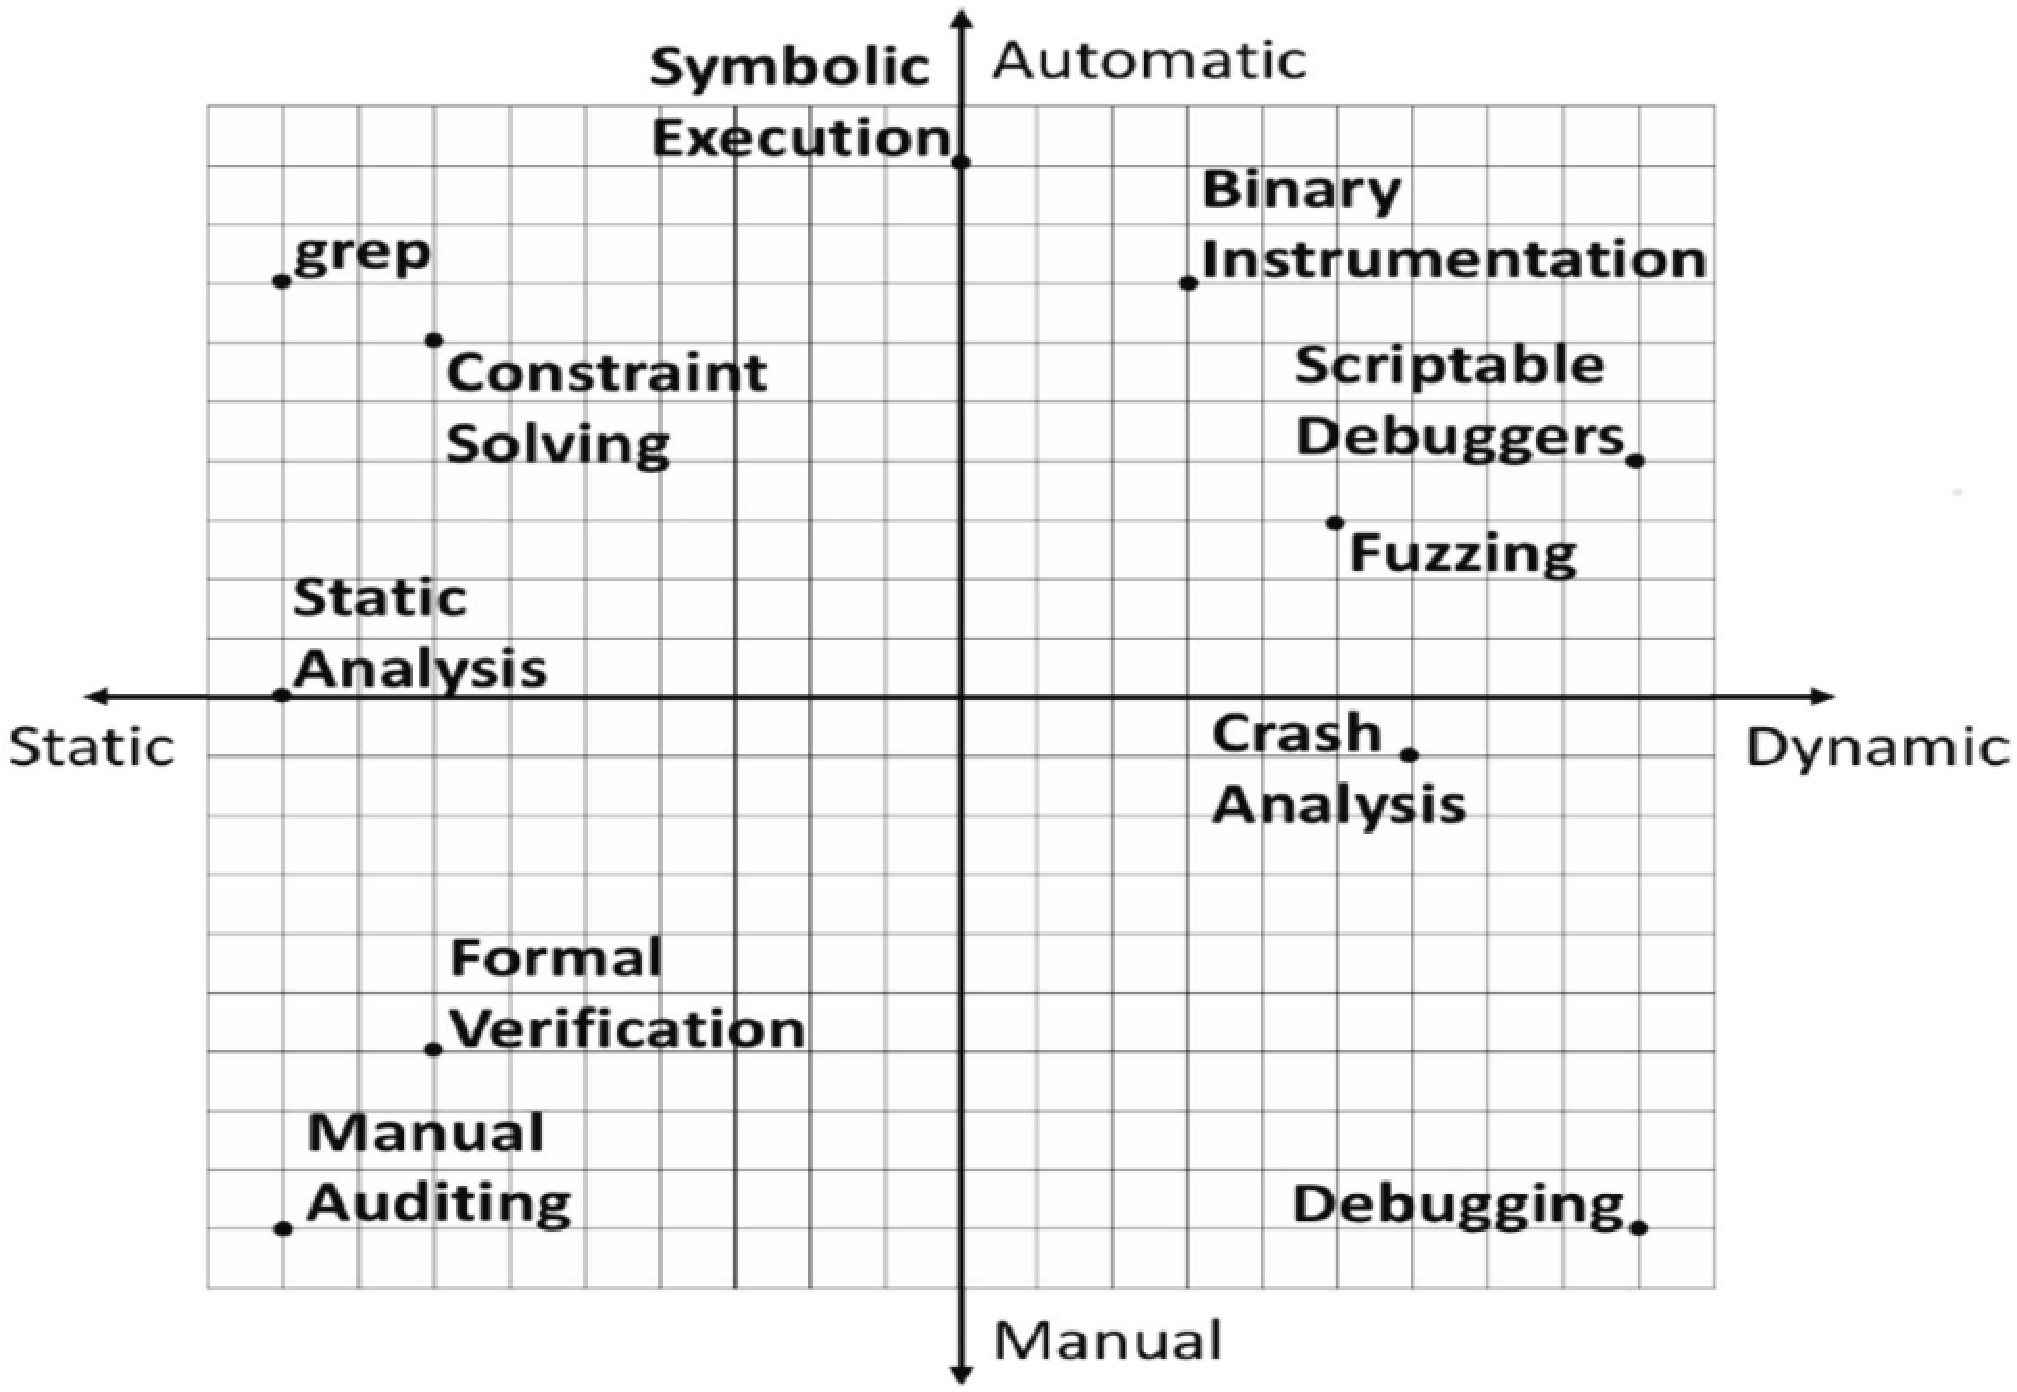
\includegraphics[width=0.6\linewidth]{img/vulnerabilities/manaut}
\end{center}
Di conseguenza, una tecnica può essere
\begin{itemize}
	\item Dinamica e automatica, esempio: binary instrumentation (inserire codice a runtime) o fuzzing (inviare input con l'obiettivo di trovare comportamenti anomali)
	\item Dinamica e manuale, esempio: debugging (eseguire il programma passo-passo per osservarne lo stato interno)
	\item Statica e manuale, esempio: manual auditing del codice (revisione manuale), verifica formale (dimostrare matematicamente la correttezza)
	\item Statica e automatica, esempio: analisi statica, esecuzione simbolica
\end{itemize}

%La symbolic execution nasce come tecnica statica, ma resa dinamica for reasons?\\

%s3?
Prima di effettuare le analisi è necessario definire delle proprietà attribuibili ai tool usati per effettuare le analisi. Le proprietà principalmente sono:
\begin{itemize}
	\item \textbf{Soundness}: una tecnica è \textit{sound} se è in grado di dire che un programma non ha nessuna vulnerabilità, ovvero se c'è una vulnerabilità la trova. Possono esserci \textbf{falsi positivi} (si tratta di un'approssimazione astratta), ma se è presente una vulnerabilità vera la trova. Di conseguenza, un programma è unsound se ci sono dei falsi negativi
	\item \textbf{Completeness}: una tecnica è \textit{complete} se, quando una vulnerabilità viene trovata, questa è vera. Può offrire \textbf{falsi negativi}, ovvero "mancare" vulnerabilità, ma se la trova è sicuramente una vulnerabilità reale. Di conseguenza, una tecnica incomplete può avere falsi positivi
\end{itemize}

\paragraph{TL;DR:} Le tecniche possono essere \textbf{sound}: trova tutti i bug possibili, potrebbe essere un falso positivo, oppure \textbf{complete}: può non trovare tutti i bug, ma se lo trova è una vulnerabilità reale. Ovviamente non esiste un tool che le ha entrambe.\\

Da queste proprietà si possono derivare altre caratteristiche, ad esempio:
\begin{itemize}
	\item se un tool è sound allora vuol dire che considera tutti i path di esecuzione possibili del programma, in quanto requisito per trovare tutti i bug possibili; in maniera dinamica questo non è fattibile, viene fatto tramite tecniche di static analysis, costruendo un'astrazione dell'esecuzione del programma
	\item se un tool è complete allora deve mostrare esecuzioni del programma che permettono di verificare le vulnerabilità; quindi l'analisi è più dinamica, il programma viene lanciato con un set di input che possono causare problemi; la tecnica fornisce input concreti che triggerano vulnerabilità
\end{itemize}
La soundness è più legata alla static analys, mentre la completeness alla dynamic analysis.\\

La \textbf{static analysis} consiste generalmente di modelli matematici astratti per l'esecuzione del programma per poi fare inferenza su quali possibili path potrebbero portare a vulnerabilità. La \textbf{dynamic analysis} invece utilizza esecuzioni più concrete per mostrare vulnerabilità effettive. Solitamente, i tool di detection hanno un approccio ibrido, usando tecniche statiche e dinamiche per ottenere un buon compromesso tra soundness e completeness. Il trade off si traduce in quanti falsi positivi e falsi negativi saranno presenti.\\

Una differenza importante tra static e dynamic execution sono le performance: la static analysis è una analisi del codice, di conseguenza è molto più veloce dell'esecuzione vera e propria del programma (la dynamic deve eseguire davvero il programma, quindi può essere molto lenta). \\

\subsection{Symbolic Execution}

La static analysis è una analisi off-line a partire da codice sorgente o binario del programma, quindi produce risultati riguardo la qualità del codice. Vengono definite delle proprietà a priori sul codice e i tool di static analysis controllano che queste vengano rispettate. \\

Un classico esempio di analisi statica è il compilatore di un programma: per la compilazione e ottimizzazione bisogna effettuare un'analisi del codice; molti tool di analisi statica si basano su ciò che produce il compilatore. L'analisi statica può usare o meno l'esecuzione simbolica.\\

La symbolic execution è una tecnica di static analysis che permette di eseguire in maniera off-line un'esecuzione del programma, "finge" un'esecuzione del programma. Si chiama "simbolica" perché vengono usati valori simbolici, viene calcolata un'approssimazione del programma per ottenere formule che rappresentano lo stato del programma in diversi punti di esecuzione. \\

%cambio slide
Il testing funziona: i bug riportati sono reali, ma ogni test è sostanzialmente un'asserzione, ogni condizione di test può controllare solo una possibile esecuzione. In breve, complete but not sound. Si spera che il caso di test generalizzi abbastanza, ma non ci sono garanzie.\\

La symbolic execution generalizza quello che è il testing di casi singoli, vuole essere "più sound", rappresentando più in generale l'esecuzione del programma. Da asserzioni su input concreti passa ad asserzioni su simboli generici, esempio: 
\begin{center}
	\texttt{assert(f(3) == 5)} $\longrightarrow$ \texttt{y = a; assert(f(y) == 2*y-1);}
\end{center}

Se il path di esecuzione dipende da variabili sconosciute, l'esecuzione simbolica viene divisa concettualmente
\begin{center}
	\texttt{int f(int x) { if (x > 0) then return 2*x - 1; else return 10; }}
\end{center}
Una "esecuzione simbolica parallela".\\

Esempio: 
\begin{center}
	\begin{minipage}{0.78\linewidth}
		\begin{minted}{c}
int a = alpha, b = beta, c = gamma; // symbolic!
int x = 0, y = 0, z = 0;
if (a) {
	x = -2;
}
if (b < 5) {
	if (!a && c) { y = 1; }
	z = 2;
}
assert(x+y+z != 3)
		\end{minted}
	\end{minipage}
\end{center}

\begin{center}
		\begin{tikzpicture}[
	level 1/.style={sibling distance=100mm},
	level 2/.style={sibling distance=70mm},
	level 3/.style={sibling distance=35mm},
	level 4/.style={sibling distance=22mm},
	]
	\node {$x=0, y=0, z=0$}
	child {
		node {$\alpha$}
		child { 
			node {$x=-2$}
			child {
				node {$\beta < 5$}
				child {
					node {$z = 2$}
					child {
						node {\color{g}$\alpha \wedge (\beta < 5)$}
					}
					edge from parent 
					node[left] {$t$}
				}
				child {
					node {\color{g}$\alpha \wedge (\beta \geq 5)$}
					edge from parent 
					node[right] {$f$}
				}
			}
			edge from parent 
			node[left] {$t$}
		}
		child {
			node {$\beta < 5$}
			child{
				node {$\neg \alpha \wedge \gamma$}
				child{
					node {$y=1$}
					child {
						node {$z=2$}
						child {
							node {\color{red} $\neg \alpha (\beta < 5) \wedge \gamma$}
						}
					}
					edge from parent 
					node[left] {$t$}
				}
				child {
					node {$z=2$}
					child{
						node {\color{g} $\neg \alpha \wedge (\beta < 5) \wedge \neg \gamma$}
					}
					edge from parent 
					node[right] {$f$}
				}
				edge from parent 
				node[left] {$t$}
			}
			child {
				node {\color{g} $\neg \alpha \wedge (\beta \geq 5)$}
				edge from parent 
				node[right] {$f$}
			}
			edge from parent 
			node[right] {$f$}
		}
	};
\end{tikzpicture}
\end{center}

Non voglio eseguire realmente il programma, ma si vuole verificare che non ci possa mai essere un'esecuzione del programma che viola determinate proprietà. Voglio vedere se esiste una classe di input che permette di violare le condizioni di esecuzione del programma.\\

\newpage

Per ogni terminazione di path di esecuzione sarà presente una \textbf{path condition}: una formula che permette di individuare tutti gli input che permettono di eseguire quel determinato path (nell'esempio: in verde se soddisfacibili, rosse altrimenti); se tutte le condizioni sono verificate (e quindi l'equazione logica è risolta) vuol dire che gli input permettono di entrare in quel determinato path di esecuzione.\\

Ogni foglia dell'albero di esecuzione ha legata la sua equazione logica che permette di stabilire i potenziali input che portano l'esecuzione in quel determinato path.\\

Se trovo una violazione delle asserzioni in un determinato path, risolvendo la path condition ottengo la classe di input che causa la violazione dell'asserzione. Dalla formula si può derivare l'input concreto per la violazione. Trovare input per la violazione diventa problema per un \href{https://en.wikipedia.org/wiki/Constraint_programming}{\texttt{constraint solver}} (come ad esempio \href{https://github.com/z3prover/z3}{\texttt{Z3}}).\\

Ogni path dell'esecuzione simbolica rappresenta più esecuzioni del programma: esattamente il set di esecuzioni i cui valori concreti soddisfano la path condition. In questo modo si possono coprire molte parti di esecuzione e testing.\\

Vista come analisi statica, la symbolic execution è
\begin{itemize}
	\item \textbf{complete}, ma \textbf{non sound} (generalmente non termina, si "incastra" spesso, la terminazione non è garantita)
	\item dipendente da path, flow e contesto
\end{itemize}

L'idea è piuttosto vecchia, ma aveva dei limiti che la rendevano poco pratica, in particolare: può essere molto compute-intensive: i path possibili possono essere \textit{tanti}, con path condition lunghe e difficili da verificare (anche solo la soddisfacibilità); quindi soggetta all'hardware del tempo: ad oggi hardware e algoritmi per i SMT/SAT solver sono molto migliorati.\\
Nel 2005-2006 è stato ripresa l'idea di symbolic execution per l'ambito del bug finding, con l'aggiunta di euristiche per ridurre lo spazio di esecuzione.\\

\newpage

\paragraph{Symbolic variables:} All'interno delle espressioni (quindi all'interno del linguaggio) vengono \textbf{aggiunte variabili simboliche}, le quali rappresentano valori sconosciuti. Vengono introdotte quando sono presenti input forniti al programma (\texttt{mmap}, \texttt{read}, \texttt{write}, \texttt{\dots}). Se un bug viene trovato queste permettono di riprodurlo. Sono dei "placeholder" per valori sconosciuti a compile time (noti solo durante l'esecuzione).\\

Vogliamo fare in modo che il linguaggio possa includere espressioni simboliche. Normalmente, le variabili in un programma contengono valori, ora possono contenere anche espressioni simboliche. \\

Esempio: 
\begin{center}
	\begin{minipage}{0.3\linewidth}
		\begin{minted}{c}
x = read();
y = 5 + x;
z = 7 + y;
a[z] = 1;
		\end{minted}
	\end{minipage}
	\hfill
	\begin{minipage}{0.6\linewidth}
		La memoria simbolica conterrà: 
		\begin{center}
			\begin{tabular}{l l l}
				\texttt{x} & $\mapsto$ & $\alpha$ \\
				\texttt{y} & $\mapsto$ & \texttt{5+$\alpha$} \\
				\texttt{z} & $\mapsto$ & \texttt{12+$\alpha$}
			\end{tabular}
		\end{center}
		E se \texttt{a} non è abbastanza grande, il valore di $\alpha$ potrebbe causare problemi.
	\end{minipage}
\end{center}

Il \textbf{controllo del programma} può essere \textbf{condizionato dai valori simbolici} (il programma dipende anche dai valori esterni, generalmente). Esempio:
\begin{center}
	\begin{minipage}{0.3\linewidth}
		\begin{minted}{c}
x = read();
if (x>5) {
   y = 6;
   if (x<3)
      y = 5;
} 
else 
   y = 0;
		\end{minted}
	\end{minipage}
\end{center}

E possiamo rappresentare l'influenza dei valori simbolici attraverso le path conditions. Esempio: l'esecuzione arriva alla riga \texttt{3} solo se la path condition $\pi = \alpha > 5$, mentre alla riga \texttt{5} si arriva solo se $\pi = \alpha > 5 \wedge \alpha < 10$.\\

%L'esecuzione del programma può essere modificata considerando le path condition. Esempio:
%s15

Una path condition può essere insoddisfacibile: \textbf{unfeasible path} (non c'è soluzione alla formula logica). Le soluzioni a path constraints possono essere usate come input concreti.\\

Si possono introdurre asserzioni che permettono di determinare se ci sono vulnerabilità sfruttando la feasibility dei path. Esempio: prima di accedere ad un array si introducono dei bound check:
\begin{center}
	\begin{minipage}{0.35\linewidth}
		\begin{minted}{c}
x = read();
y = 5 + x;
z = 7 + y;
if(z < 0)
   abort();
if(z >= len(a));
   abort();
a[z] = 1;
		\end{minted}
	\end{minipage}
\end{center}

Le due condizioni permettono di controllare non ci siano buffer overflow all'interno del programma. Trovare delle soluzioni alle path condition rilevanti (nell'esempio, per la riga \texttt{5} $\pi  =12 + \alpha < 0$ e \texttt{7} $\pi = \neg (12 + \alpha < 0) \wedge 12 + \alpha \geq 4$) vuol dire trovare classi di input che permettono di avere la vulnerabilità per cui si sta testando (buffer overflow in questo caso).\\

Ogni volta che si presenta un branch si ha una fork dell'esecuzione simbolica: si ha un symbolic executor per ogni path di esecuzione. Accade quando si possono avere soluzioni sia alla path condition che alla sua negazione. \\

\paragraph{Libraries e codice nativo:} L'esecuzione simbolica prima o poi raggiungerà i "limiti" dell'applicazione: librerie, sistema o chiamate a codice assembly. Le soluzioni a questo problema possono essere: 
\begin{itemize}
	\item far entrare il symbolic executor nella libreria, ma potrebbero essere \textit{molto} complicate (probabilmente si incastrerà)
	\item fornire un modello delle librerie per l'esecuzione
\end{itemize}

\newpage

\subsubsection{Concolic Execution}

Anche chiamata \textbf{dynamic symbolic execution}, il nome viene da concrete+symbolic. Lavora con gli stessi concetti della symbolic execution ma è un ibrido tra analisi statica e dinamica. \\

Si instrumenta il programma per fare symbolic execution durante l'esecuzione: a partire da un input concreto si esegue il programma, ma si traccia l'esecuzione simbolica durante l'esecuzione concreta; si tiene traccia delle path condition (shadow memory). Ogni volta che si trova un ramo condizionale nel flusso di controllo si tiene traccia del ramo percorso concretamente e la condizione per percorrerlo.\\

Terminata l'esecuzione di un percorso, si ottiene una path condition "completa", per generare un percorso alternativo da eseguire si nega una delle condizioni e si usa un constraint solver per trovare un nuovo input che soddisfa tali condizioni.\\

Si esplora un percorso alla volta tramite valori concreti. Permette di avere sempre dei valori concreti per ogni esecuzione e si possono anche seguire chiamate esterne al programma (perdendo symbolic-ness). Si possono gestire casi senza necessariamente far esplodere la complessità per il SMT solver.\\

% End L9